\documentclass[tikz,border=5mm]{standalone}
\usetikzlibrary{decorations.markings}

\begin{document}
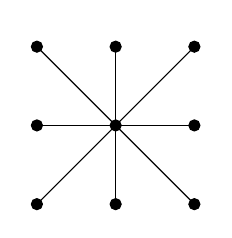
\begin{tikzpicture}[every loop/.style={min distance=30mm}]

    % these are the vertices
    \draw[fill=black] (3,3) circle (2pt) node[above] {};
    \draw[fill=black] (2,3) circle (2pt) node[above] {};
    \draw[fill=black] (1,3) circle (2pt) node[above] {};
    \draw[fill=black] (3,2) circle (2pt) node[above] {};
    \draw[fill=black] (2,2) circle (2pt) node[above] {};
    \draw[fill=black] (1,2) circle (2pt) node[above] {};
    \draw[fill=black] (3,1) circle (2pt) node[above] {};
    \draw[fill=black] (2,1) circle (2pt) node[above] {};
    \draw[fill=black] (1,1) circle (2pt) node[above] {}; 

    \draw (2,2) -- (3,3);
    \draw (2,2) -- (2,3);
    \draw (2,2) -- (1,3);
    \draw (2,2) -- (3,2);
    \draw (2,2) -- (1,2);
    \draw (2,2) -- (3,1);
    \draw (2,2) -- (2,1);
    \draw (2,2) -- (1,1);

\end{tikzpicture}
\end{document}
